%ब
\section{Solution4:  Metadata Cluster} \label{s:design-sol4}

In this solution,  metadata  is saved in a separate column family,  which is
similar to Solution~3 (Figure~\ref{fd:Metadata-Solution3}). 
However,  in this solution,  the \texttt{Metadata} column family is saved in a
separate Cassandra cluster instead of saving the metadata as a column family
within the same keyspace.  This means that the metadata storage
is decentralised and separated from the Cassandra cluster containing the
keyspace with actual data. 
Metadata  is not as widely replicated as in the previous solutions since the
replication of \texttt{Metadata} is only within the metadata cluster. 
Figure~\ref{fd:MetadataCluster-Solution4} shows an example of how the University
keyspace is saved in a separate cluster (nodes \texttt{A}, \texttt{B}, 
\texttt{C},  \texttt{D}) and the metadata is saved in the separate cluster called
Metadata cluster (nodes \texttt{L}, \texttt{M}, 
\texttt{N},  \texttt{O}).  
In this example,  the metadata column family \texttt{Metadata} is
inserted into \texttt{MetadataCluster},  while the column
families \texttt{Student},  \texttt{course} and \texttt{Enrolment} are entered
into another cluster,  namely \texttt{KeyspaceCluster}. 

% The Cassandra cluster is named ‘Test Cluster’ and consists
% of the nodes that have Cassandra with the entity column families (Student, 
% Course,  and Enrolment).  A separate cluster called “Metadata Cluster” consists of
% nodes that have only the metadata column families. 
\begin{figure}[h]
	\centering
	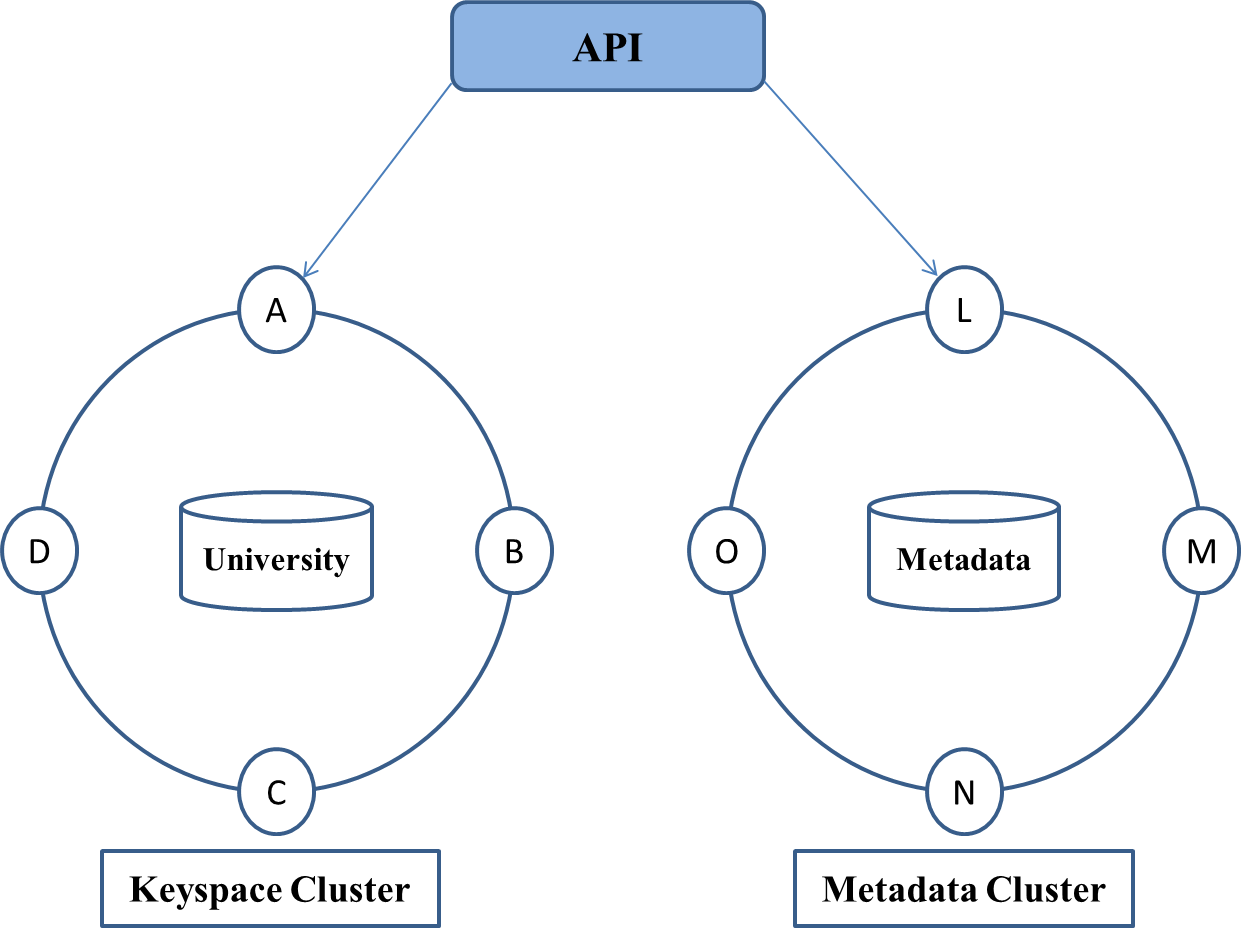
\includegraphics[width=.6\textwidth]{./figure/Solutions/Sol4-cluster-pic.png}
	\caption{Metadata Cluster in Solution
	4}\label{fd:MetadataCluster-Solution4}
	
\end{figure}
 The experimental \ac{API} connects to the Metadata cluster as well as
the cluster containing the keyspace to perform any operations on the actual
data.  Whenever a \ac{CRUD} operation is invoked on a column family,  the
experimental \ac{API} accesses its relevant metadata and caches it to re-use it
for future operations on this column family. 
Additionally,  the experimental \ac{API} can perform validations without
disruptions using the cached metadata when the metadata cluster is unresponsive or not active . 
Having metadata in a persistence layer is effective since metadata is not
expected to be as frequently changed as the actual data.  This also saves
operational time by not having to connect to the
\texttt{Metadata} column family each time  metadata is accessed. 


% As of now,  ‘Test Cluster’ is the name of the cluster for all the entity column
% families existing on Cassandra nodes.  Some of the Cassandra nodes are
% Saddleback,  meow,  Marrakech etc.  located in the ECS labs.  To have a separate
% cluster of nodes for Metadata,  it was required that the Cassandra configuration
% files were changed.  This involved changing the listening port,  RPC port,  and TCP
% port to different values from that of the ‘Test Cluster’.  It was also necessary
% to change the path configurations for the saved caches and log files so that it
% does not overwrite the files of the ‘Test Cluster’. 


% Just as in other solutions,  metadata information needs to be checked during
% any database operations.  Every time a referential integrity check is
% performed,  the API connects to the ‘Metadata Cluster’ and retrieves the
% metadata information. 
% Connection pools are maintained to reuse the connections whenever needed.  In
% order to perform the database operations,  the API then connects to the ‘Test
% Cluster’ on any of its nodes.  For example,  if an insert operation is invoked
% on Enrolment,  it is necessary to check if the foreign keys for Student and
% Course column families exist in their respective parent column families.  The
% details of the referenced column families are retrieved from the Metadata
% column family in the ‘Metadata Cluster’.  Once this information is processed, 
% the API connects to the referencing column families in the ‘Test Cluster’ and
% completes the insert operation. 
This  approach is very useful when an application handles multiple keyspaces
and have to store and maintain metadata (which can be large) for its several
keyspaces. 
In such cases it is straightforward and simple to maintain all the metadata  in a
separate cluster  decoupled from the actual data and avoids having to handle
the actual data. 
% Even if the metadata
% cluster is unresponsive or not active the \ac{API} can perform operations with 
% the cached metadata. 
 
 This approach is inspired from the way most distributed systems
 save metadata in \ac{MDS} clusters (Lin Xia et al.  2009). 
 For better scalability and efficient access of metadata,  \ac{MDS} are
 often separate clusters in large distributed environments.  In distributed
 systems such clusters  have a master \ac{MDS} and subordinate \acp{MDS},  with
 each server running on a different node.  But in this solution such delegations
 of tasks are not required since all nodes in a Cassandra cluster  have the same
 responsibilities and do not have a master-slave configuration.  This solution
 thus adopts the design of having a cluster of dedicated nodes to save metadata
 information and to have a central location to preserve and maintain metadata
 for many keyspaces. 
 